\documentclass{article} % For LaTeX2e
\usepackage[legalpaper, margin=0.5in]{geometry}
\usepackage{amsmath}
\usepackage{amsfonts,dsfont}
\usepackage{amssymb}
\usepackage[ruled,vlined]{algorithm2e}

\usepackage{graphicx}
\usepackage{caption}
\usepackage{subcaption}
\usepackage{xcolor}

\begin{document}

\section{Histogram of Angle Distributions for IFOR}
The below figure shows that ${\mathbf w}_{unif}$ tends to have a smaller angular separation from the normalized IFOR score vectors of anomalies than from those of nominals.
\begin{figure}[h]
	\centering
	\captionsetup{labelformat=empty}
	\begin{subfigure}[b]{0.23\textwidth}
		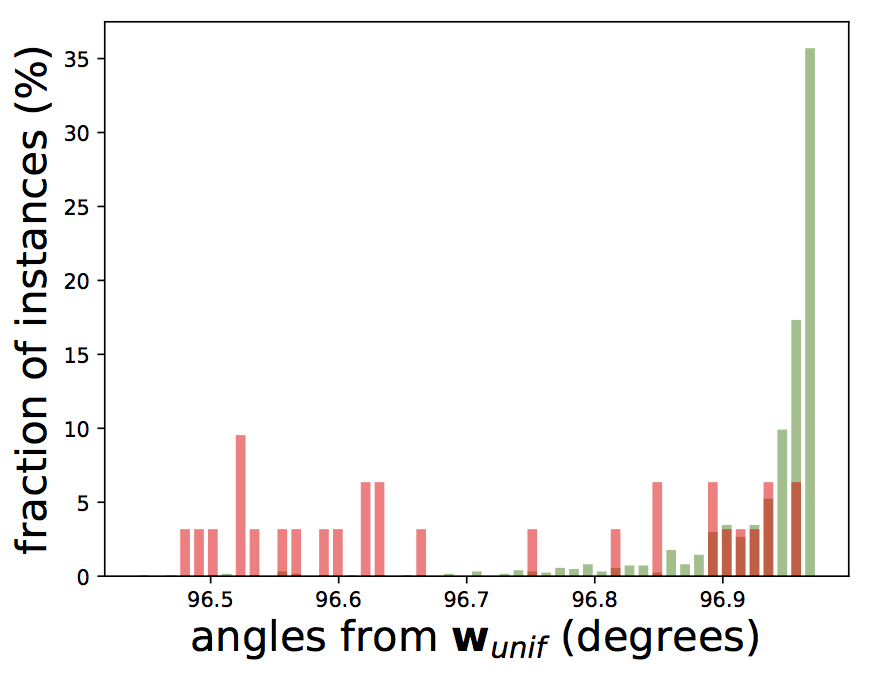
\includegraphics[width=\textwidth]{angles/angles_abalone_iforest.png}
		\caption{Abalone}
		\label{fig:angles_abalone}
	\end{subfigure}
	~
	\begin{subfigure}[b]{0.23\textwidth}
		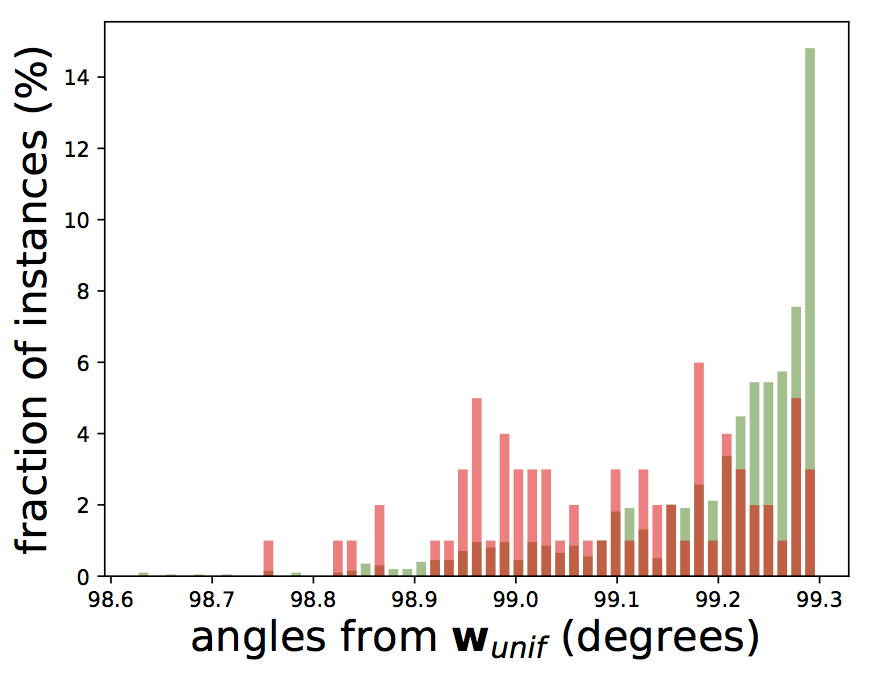
\includegraphics[width=\textwidth]{angles/angles_ann_thyroid_1v3_iforest.png}
		\caption{ANN-Thyroid}
		\label{fig:angles_ann_thyroid_1v3}
	\end{subfigure}
	\begin{subfigure}[b]{0.23\textwidth}
		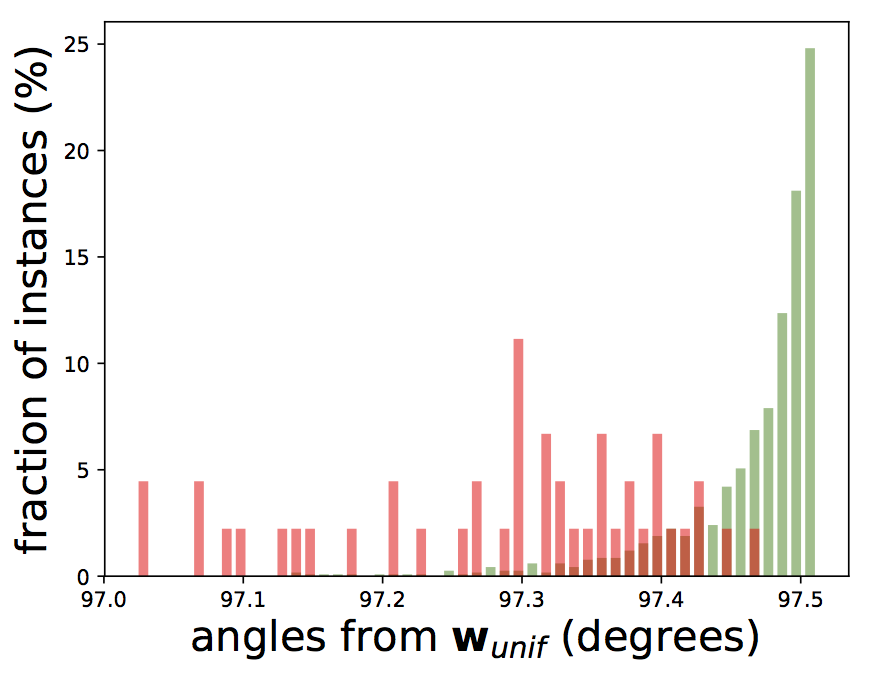
\includegraphics[width=\textwidth]{angles/angles_cardiotocography_1_iforest.png}%
		\caption{Cardiotocography}
		\label{fig:angles_cardiotocography}
	\end{subfigure}
	~
	\begin{subfigure}[b]{0.23\textwidth}
		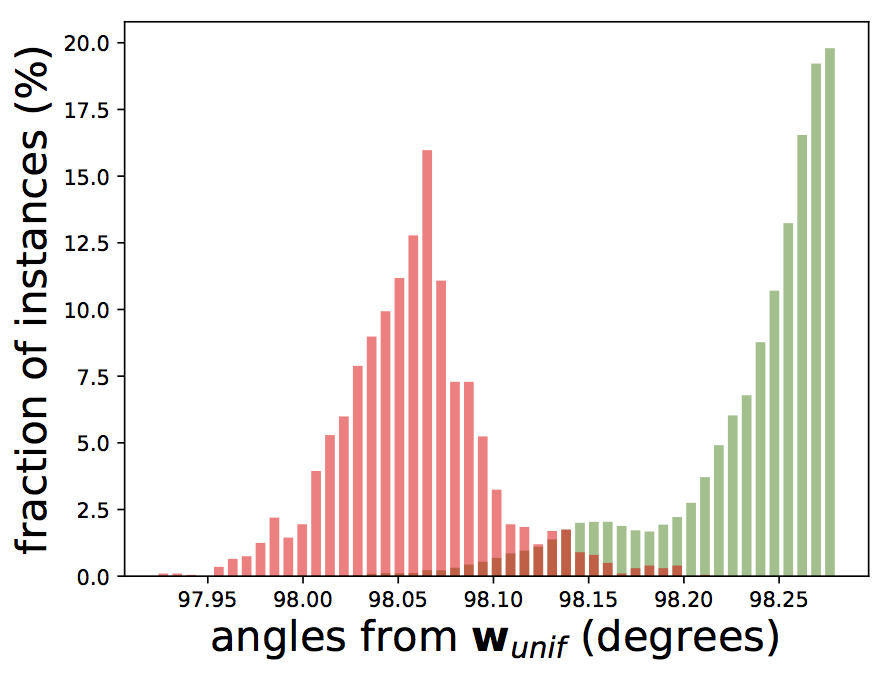
\includegraphics[width=\textwidth]{angles/angles_covtype_iforest.png}
		\caption{Covtype}
		\label{fig:angles_covtype}
	\end{subfigure} \\
	\begin{subfigure}[b]{0.23\textwidth}
		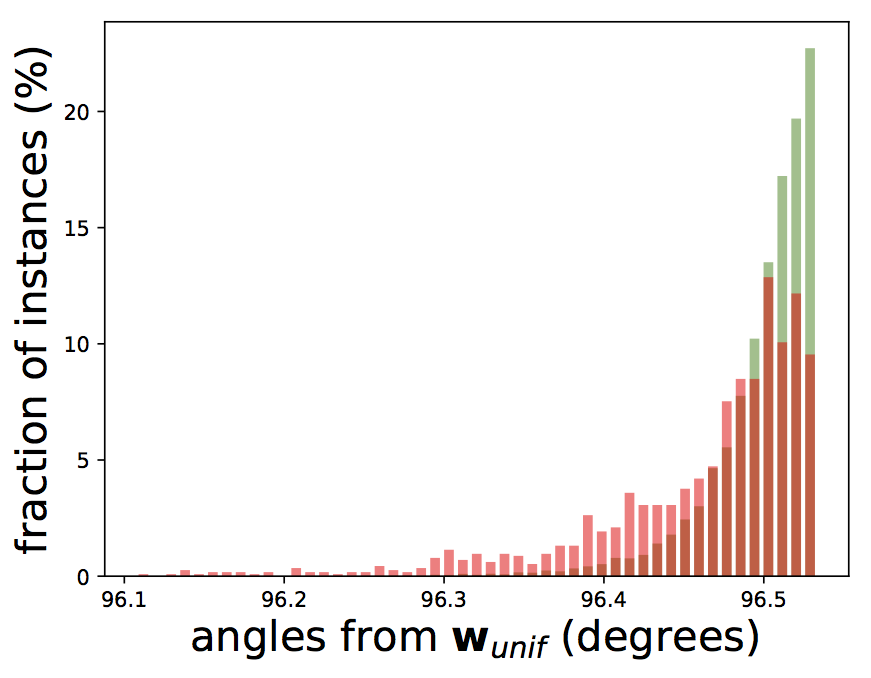
\includegraphics[width=\textwidth]{angles/angles_electricity_iforest.png}
		\caption{Electricity}
		\label{fig:angles_electricity}
	\end{subfigure}
	~
	\begin{subfigure}[b]{0.23\textwidth}
		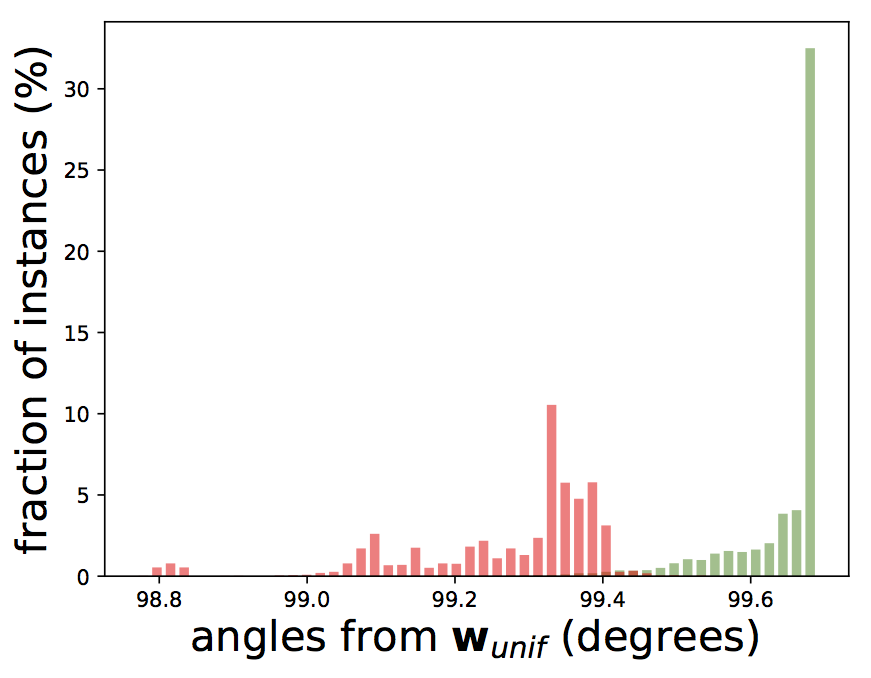
\includegraphics[width=\textwidth]{angles/angles_kddcup_iforest.png}
		\caption{KDDCup99}
		\label{fig:angles_kddcup}
	\end{subfigure}
	~
	\begin{subfigure}[b]{0.23\textwidth}
		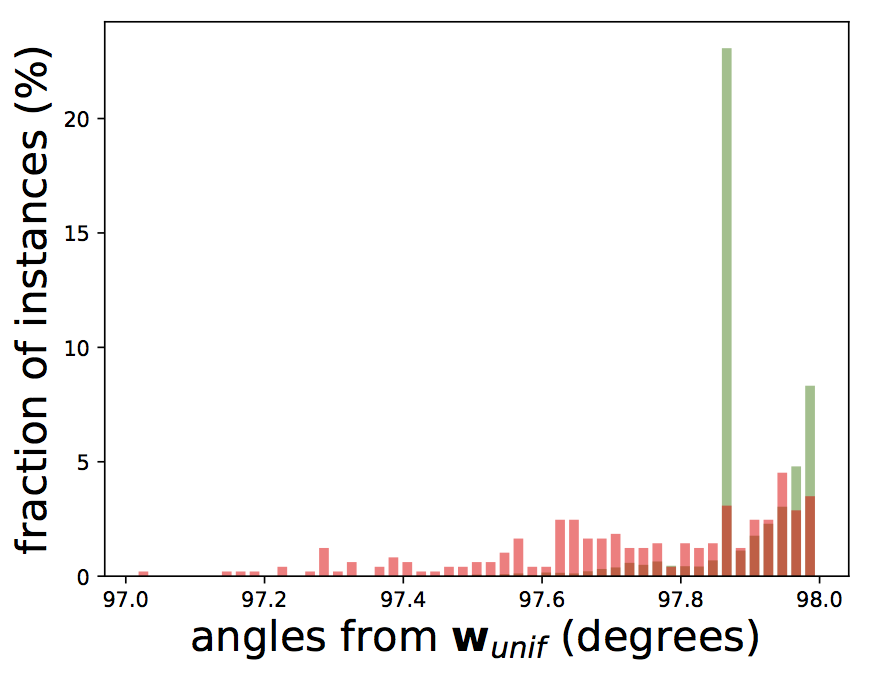
\includegraphics[width=\textwidth]{angles/angles_mammography_iforest.png}
		\caption{Mammography}
		\label{fig:angles_mammography}
	\end{subfigure}
	~
	\begin{subfigure}[b]{0.23\textwidth}
		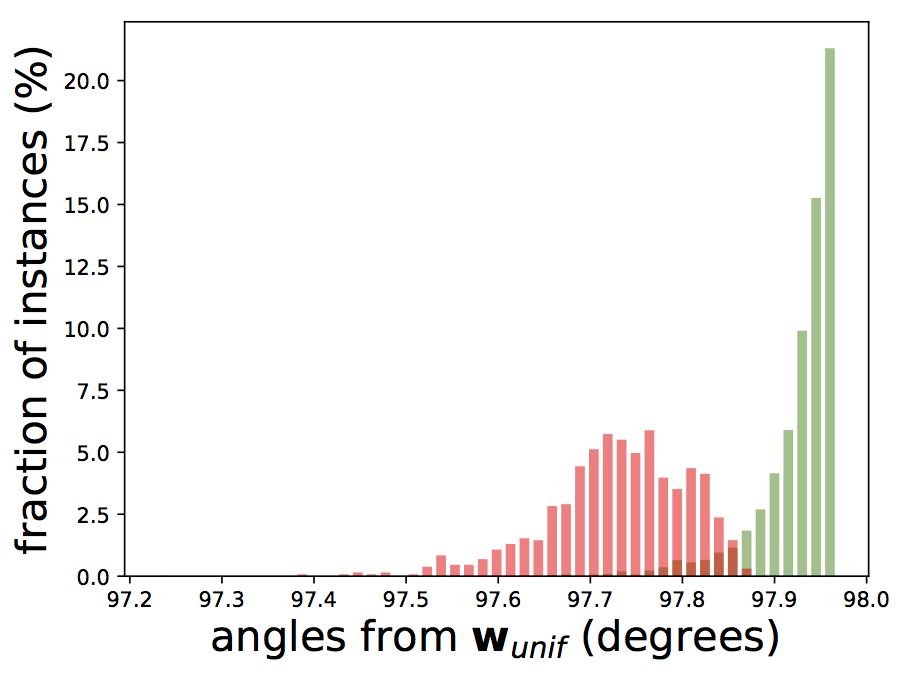
\includegraphics[width=\textwidth]{angles/angles_shuttle_1v23567_iforest.png}
		\caption{Shuttle}
		\label{fig:angles_shuttle}
	\end{subfigure} \\
	\begin{subfigure}[b]{0.23\textwidth}
		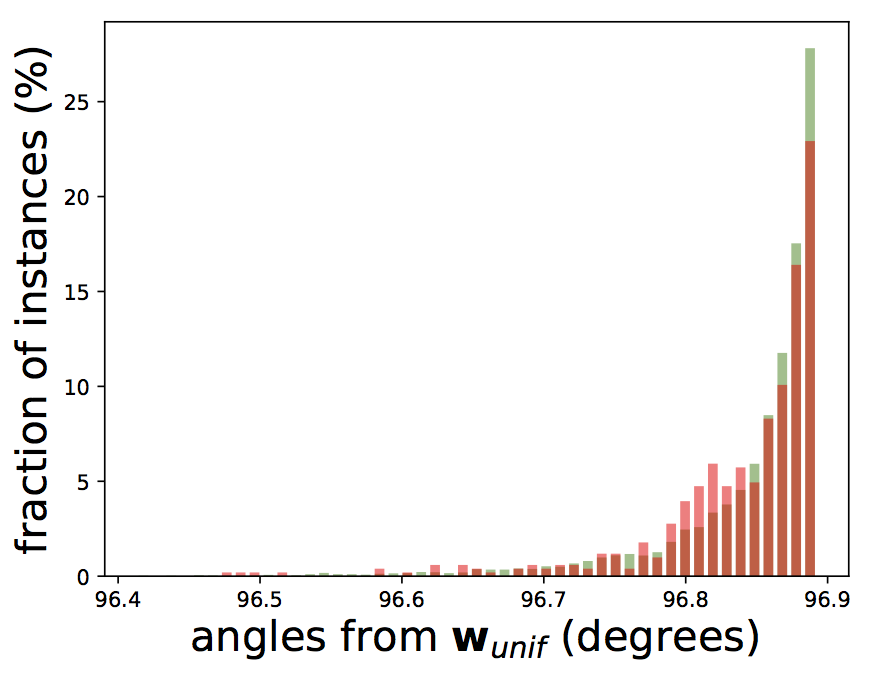
\includegraphics[width=\textwidth]{angles/angles_weather_iforest.png}
		\caption{Weather}
		\label{fig:angles_weather}
	\end{subfigure}
	~
	\begin{subfigure}[b]{0.23\textwidth}
		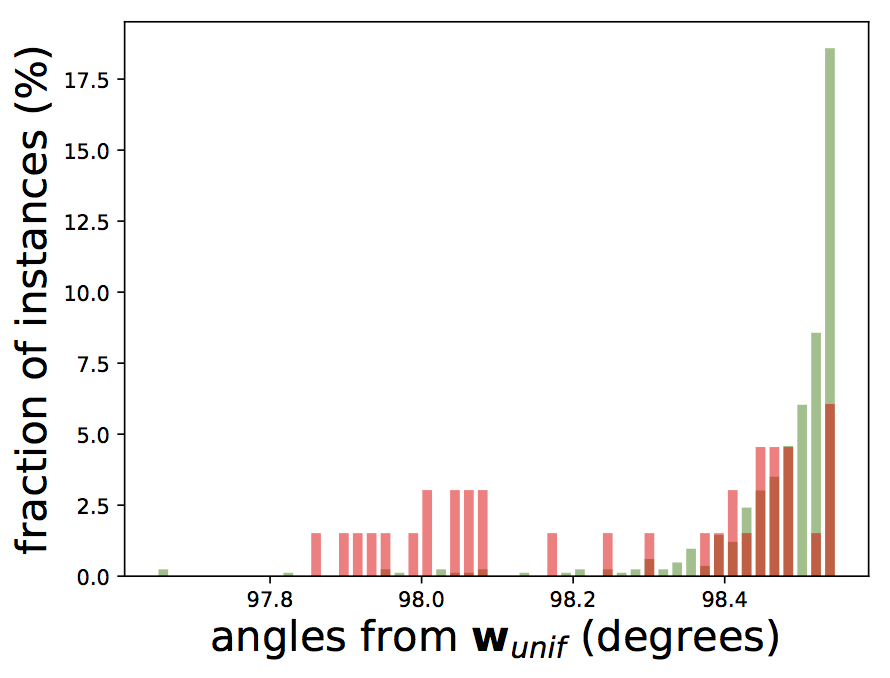
\includegraphics[width=\textwidth]{angles/angles_yeast_iforest.png}
		\caption{Yeast}
		\label{fig:angles_yeast}
	\end{subfigure} \\[-1ex]
	\caption{Histogram distribution of the angles between score vectors from IFOR and ${\mathbf w}_{unif}$. The red and green histograms show the angle distributions for anomalies and nominals respectively. Since the red histograms are closer to the left, anomalies are aligned closer to ${\mathbf w}_{unif}$. Prior research has shown that \textit{Weather} and \textit{Electricity} are hard (Wu et al. 2014) and this is reflected in figures {\bf (e)} and {\bf (i)}.}
	\label{fig:angles_all}
\end{figure}

\end{document}
